\chapter{Prototypen} 
In diesem Kapitel entstehen Prototypen, die Renew schrittweise modularisieren bis diese den größten Teil ihre Funktionalität auf dem Modulpfad betreiben kann. 


Für die Umsetzung werden zuerst Anforderungen erfasst, die der modularisierte Renew Prototyp erfüllen müsste um unserer Vision der Implementation zu entsprechen. Infolgedessen entsteht ein Implementierungsplan sowie ein Prototyp. 

%Anforderungen an System 
\section{Anforderungen} \label{sec:anforderungen}
Im Kern der Modernisierung von Renew liegt die Anpassung von Renew an das Modulsystem von Java und dessen Anforderungen an Applikationskomponenten. Aus den Renew Plugins sollen Module entstehen, die als explizite Module auf dem Modulpfad betriebsfähig sind. Die Drittanbieter-Bibliotheken sollen mit in den Modulpfad aufgenommen werden und als automatische Module ihre Aufgabe erfüllen. Zusätzlich darf die Migration und damit verbundene Anpassung und Aufbereitung der Mängel die Kommunikation sowie interne Funktionsweise von Renew nicht verändern. Dementsprechend soll garantiert werden, dass die darunter liegende theoretische Grundlage in Takt bleibt. 

%was soll der Prototyp leisten 
\subsection{Interaktion}
Der erste modulare Renew Prototyp soll mit einer minimalen Plugin Anzahl auf dem Modulpfad betriebsfähig sein und eine Möglichkeit bieten Petrinetze zu erstellen, zu simulieren und zu serialisieren. Das heißt, es muss eine UI zu sehen sein, die mit den nötigen Werkzeugen und der darunter liegender Logik ausstattet ist. 

\subsection{Projektstruktur}
Für die Umsetzung des modularen Renew's wird für jedes Plugin eine moderne Projektstruktur benötigt, die den Inhalt entsprechend dem etablierten Maven Standardverzeichnislayout auf Java Module und die dafür benötigten Ressourcen aufteilt. 

\subsection{Entwicklungsumgebung} 
In der existierenden Renew Entwicklungsumgebung werden alle Plugin Projekte durch eine versteckte \textit{.project} beschrieben. Das heißt, der Klassenpfad und die binden der Codebausteine geschieht versteckt und für den Entwickler schwer zugänglich. Es liegt ein weiter und verschachtelter Weg der Eclipse Konfiguration-UI, die sich mit der Zeit verändern kann. Dieser Umstand wurde von mir im letzten Projekt beobachtet und kostete Zeit für alle Projektteilnehmer, da die Universitätsrechner strikten Rechten unterliegen, die keine eigen Eclipse Entwicklungsumgebung aufsetzen lässt. Darüber hinaus ist die Konfiguration von Renew in anderen Entwicklungsumgebungen wie IDEA oder Netbeans mit der \textit{.project} Konfigurationsdatei nicht möglich.
\bigbreak

Um eine Entwicklungsumgebung unabhängige Konfiguration anzulegen wird ein neues Werkzeug benötigt. 

\subsection{Packaging}
Da die Umstrukturierung von Renew an das Modulsystem durchgeführt werden muss, muss das für die Kompilation und Verpacken der Codebasis verantwortliche Werkzeug die Veränderung miterleben. 


Renew benutzt zur Zeit das \textit{Apache Ant} Werkzeug, dass alle Plugins kompiliert und in einer ausführbare Form bringt. Dieses ist in Jahre gekommen und enthält wesentlich geringeren Funktionsumfang gegenüber der Aktuellen Konkurrenz, wie Maven und Gradle. Diese bieten eine Abhängigkeitsverwaltung, konfigurierbare Plugins und sogar eine Programmiersprache. Im Gesetz zu der aufgeblasenen XML-Konfiguration von Ant, beherrschen die modernen \textit{build} Werkzeuge die Komplexität durch den \textit{Convention over Configuration} Ansatz und flexiblen Ausdrucksweisen. 
\bigbreak

Die minimalen Version von Renew soll sich an einem modernen \textit{build} Werkzeug bedienen und eine Ausführbares Ergebnis erzielen.


% wie setze ich die Anforderungen um 
\section{Spezifikation}
Um die Anforderungen umzusetzen, wird die erarbeitete minimale Version isoliert, umstrukturiert und mit dem Gradle \textit{build} Werkzeug für das Arbeiten in der Entwicklungsumgebung IDEA aufgerüstet. Da Gradle die Verwaltung des Projekts sowie das Kompilieren und Erstellen von ausführbaren Paketen übernehmen kann, ist es eine gute Wahl für das Aufsetzen einer modernen modularen Projektstruktur mit einem aufstrebenden Werkzeug. 


Dafür muss das bestehende Ant \textit{build} System analysiert und mit dem Gradle Werkzeug aufgebaut werden. Dieses soll so gut wie möglich die bestehende Drittanbieter-Bibliotheken verwalten, Module Kompilieren und die benötigten Erweiterungen, wie das JavaCC Werkzeug, unterstützen.  
\bigbreak

Nachdem die Projektstrukturen die passende Form angenommen haben, müssen die Projekt Abhängigkeiten analysiert und innerhalb der \textit{module-info.java} aufgenommen werden. 
\bigbreak

Zu Letzt entsteht ein bekannte Ordnerstruktur mit Drittanbieter-Bibliotheken, Plugins und Konfigurationsdateien, die  über den \textit{Plugin Manager} verwaltet werden. 

% was werde ich tun um die Spezifikation zu erfüllen 
\section{Entwurf}
Der Entwurf berücksichtigt die schrittweise Migration und lässt die Renew Applikation während der Gesamtmigration betriebsfähig bleiben. Das heißt, Plugins auf den Klassenpfad sowie Modulpfad können nahtlos mit einander kommunizieren und ihre Funktion während der Migration weiterhin erfüllen.   
\bigbreak

% Grobe darstellung der Projketstruktur als baum 
Für den ersten Prototypen wird zuerst eine, Projektstruktur erstellt die für jedes Plugin Projekt die Möglichkeit bieten soll aus mehreren Modulen zu bestehen. Dafür wird eine Struktur \ref{fig:projektstruktur} erstellt, die im Java Verzeichnis alle Module bündelt, die über den Modulnamen disjunkt von einander verwaltet werden. Nichtsdestotrotz gehören sie zum gleichen Projekt und teilen unter sich das Ressourcen Verzeichnis, das im weiteren Verlauf zum erstellen der ausführbaren Pakete benötigt wird.

\begin{figure}[h!]
  \centering
  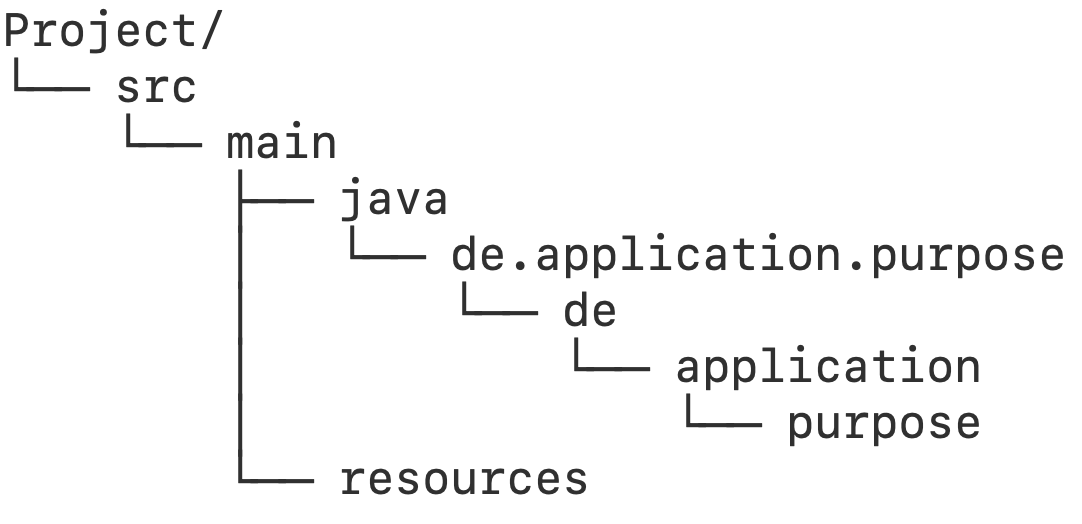
\includegraphics[width=0.6\textwidth]{material/images/project-structure.png}
  \caption{Projektstruktur}
  \label{fig:projektstruktur}
\end{figure}
       
% Wie das Gradel build system alles zusammenhalten. 
Nachdem die Projektstruktur unseren Wünschen entspricht, muss diese in der Gradle Konfigurationsdateien verankert werden. Hierfür halten wir für jedes Projekt die Projektstruktur und dessen Abhängigkeiten in der \textit{build.gradle} Konfigurationsdateien fest, indem wir Java- sowie Ressourcen-\textit{sourceSets} definieren und Projekt sowie Drittanbieter-Bibliotheken Abhängigkeiten für den  Kompilation-Pfad bestimmen.

\begin{figure}[h!]
  \centering
  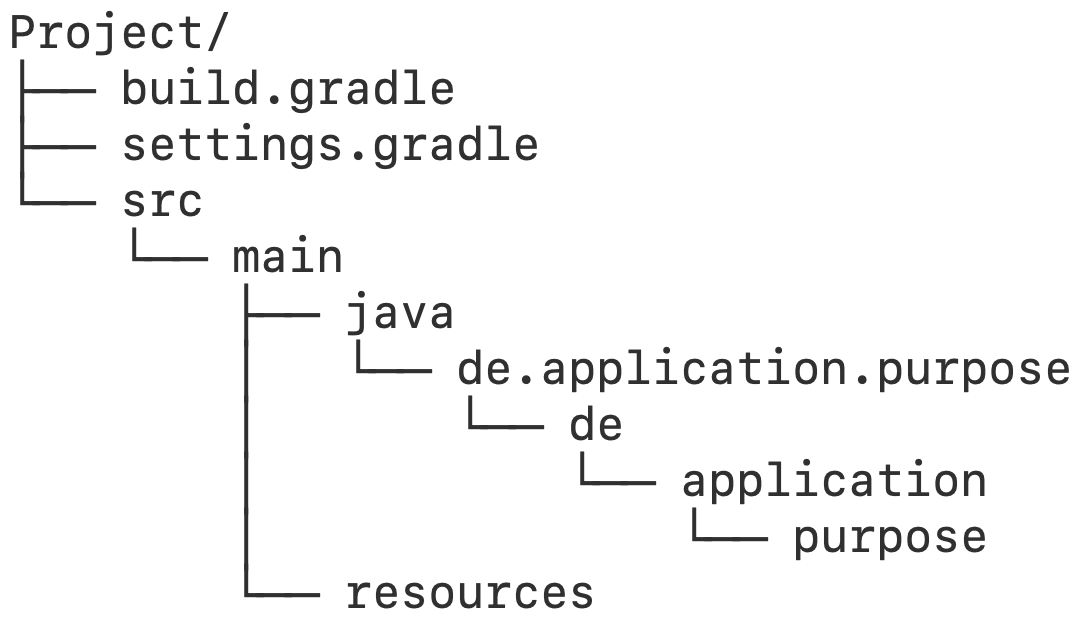
\includegraphics[width=0.6\textwidth]{material/images/gradle_project.png}
  \caption{Gradle Konfiguration}
  \label{fig:gradle_project}
\end{figure}

 Die oben genannten Schritte müssen für jedes Projekt, das für die minimal Version von Renew auserwählt wurde durchgeführt und im Anschluss über die entsprechende Entwicklungsumgebung  validiert werden. Wenn diese alle Klassen und die benötigten Abhängigkeiten finden und kompilieren kann, haben wir alle Projekte richtig strukturiert, definiert und mit einander sauber verbunden. In diesem Zustand ist die komplette Struktur des Projekts innerhalb Gradle verpackt und kann von jeder Entwicklungsumgebung ausgelesen werden. 


% Modualisierungsiddee wie ich vorgehn werden(BottomUP). 
Da jetzt eine lauffähige minimale Renew Version für den Klassenpfad erstellt werden kann, ist es Zeit diese zu Modularisieren und die einzelnen Plugins auf den Modulpfad zu migrieren. Dafür werde ich den in dem Kapitel Migration \ref{sec:bottomUP} vorgestellten \textit{bottom up} Ansatz verwenden. 

\begin{figure}[h!]
  \centering
  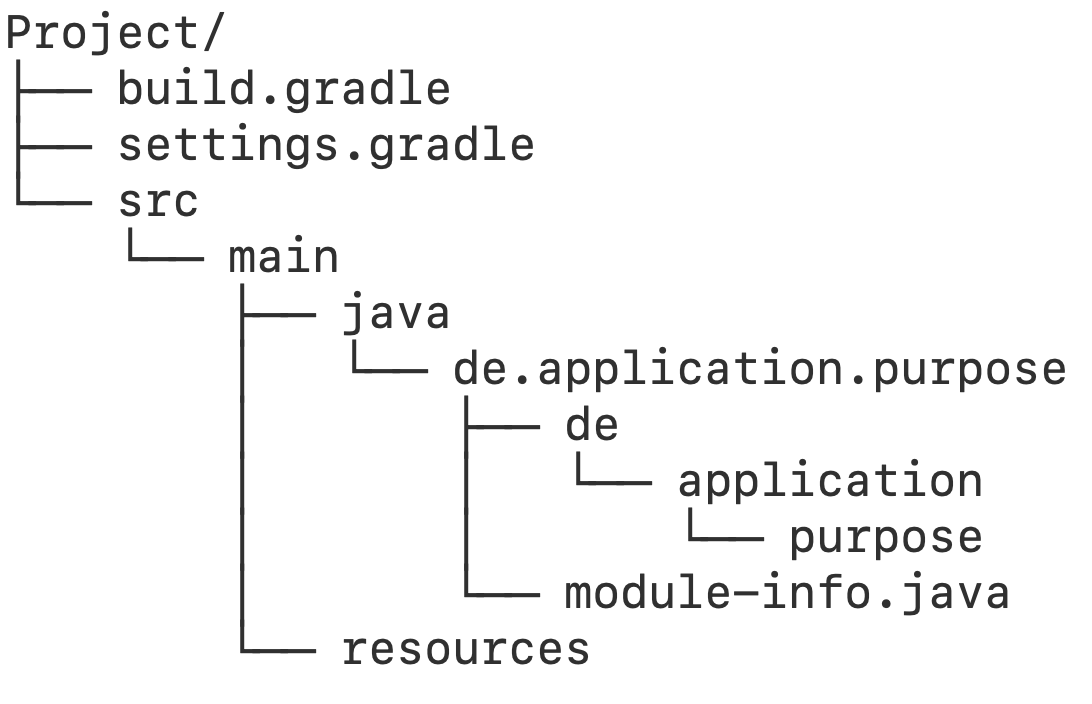
\includegraphics[width=0.6\textwidth]{material/images/module_project.png}
  \caption{Modulumwandlung}
  \label{fig:module_project}
\end{figure}

Zuerst werden die Drittanbieter-Bibliotheken, wie \textit{log4j}, auf den Modulpfad migriert und werden somit aus den Klassen- sowie Modulpfaden für die Nutzung zugleich erreichbar sein. Anschließend werden Module migriert, die keine Plugin Abhängigkeiten benötigen und aus dem Modulpfad keine Zugriffe auf den Klassenpfad ausführen, wie zum Beispiel das \textit{Util} Plugin. 
Damit diese auf dem Modulpfad ausführbar sind, werden sie durch eine \textit{moduel-info.java} Konfigurationsdateien erweitert. Diese muss sich im Stammverzeichnis des Moduls befinden wie in der Abbildung \ref{fig:module_project} dargestellt und deklariert die benötigten automatischen Module. In den nächsten Schritten werden Plugins Schritt für Schritt auf den Modulpfad migriert, indem für jedes Plugin eine eigene \textit{module-info.java} Konfigurationsdateien angelegt wird, in der sich ihre Abhängigkeiten auf automatische Drittanbieter-Module sowie explizite Plugin-Module befinden.


Diese Vorgehen wird solange durchgeführt bis jedes Plugin sich auf dem Modulpfad befindet. 


\section{Umsetzung}



\section{Evaluation}


%eine Anforderungsmenge die von mehreren Prototypen umgesetzt wird 


% Dafür wir diese von dem Rest des Systems isoliert und auf Kompilation sowie Laufzeit Abhängigkeiten untersucht. $